\documentclass[../../main.tex]{subfiles}

\begin{document}

\subsection{Reellwertige Funktionen}

Die wichtigste Eigenschaft einer Abbildung ist ihre Abbildungsvorschrift. Du weißt bereits, wie sich Abbildungsvorschriften beschreiben lassen und wie du dir Abbildungen graphisch vorstellen kannst. Mithilfe des Abbildungsgraphen, der in einem vorherigen Abschnitt erklärt wurde, können diese Vorschriften sehr gut veranschaulicht werden.

In diesem Abschnitt werden die Abbildungsvorschriften weiter untersucht: Du lernst Begriffe kennen, mit denen sich Abbildungsvorschriften beschreiben lassen und mit denen sie sich besser verstehen lassen. 

Mittlerweile solltest du gut verstanden haben, was eine Abbildung ist. Man findet oft einen zweiten Begriff, der genau dasselbe meint: Statt von einer Abbildung zu sprechen kannst du auch den Begriff \textbf{Funktion} verwenden. Beide Begriffe meinen genau das gleiche. Der Begriff Funktion ist tatsächlich sogar gebräuchlicher und wird aus diesem Grund ab und zu in diesem Kapitel verwendet. Gerade in den folgenden Kapiteln ist dann nur noch von Funktionen die Rede. Infolgedessen gibt es auch eine kompaktere Bezeichnung für das Bild $f(x)$, auf das ein Argument $x$ durch die Anwendung von $f$ abgebildet wird: Man nennt $f(x)$ auch den \textbf{Funktionswert von $f$ an der Stelle $x$}.

Während es in den einführenden Abschnitten sehr wichtig war, zu erwähnen, welche Abbildung welche Definitions- und Bildmenge hatte (weil diese wegen der vielen anschaulichen Beispiele immer unterschiedlich waren), rückt die Frage, welche Definitions- und Bildmenge eine Abbildung hat, ab sofort eher in den Hintergrund. 

Wenn nichts anderes gesagt ist, wird deshalb ab sofort davon ausgegangen, dass eine Abbildung einfach Zahlen auf Zahlen abbildet. Jede Abbildung, bei der Definitions- und Bildmenge nicht in der Schreibweise $f\colon U\rightarrow V$ angegeben sind, sondern weggelassen werden, soll einfach als eine Abbildung von den reellen Zahlen in die reellen Zahlen, also als eine Abbildung $f\colon\Real\rightarrow\Real$ verstanden werden.

\begin{example}{}
    \parpic[r]{
        \begin{tikzpicture}
            \begin{axis}[defgrid, domain=0:3, y=.8cm, x=.8cm, ymin=0, ymax=2, xmin=0, xmax=3, samples=2, ylabel=$f(x)$, xlabel=$x$]
                \addplot[color=violet] expression{(x+1)/2};
            \end{axis}
        \end{tikzpicture}
    }
    Die Abbildung (oder Funktion) $f(x)=\frac{1}{2}(x+1)$, die den rechts abgebildeten Abbildungsgraphen besitzt, bildet reelle Zahlen auf reelle Zahlen ab. Wir sparen es uns allerdings ab sofort, dies durch die Schreibweise $f\colon\Real\rightarrow\Real$ aufzuschreiben, sondern nehmen an, dass dies einfach der Normalfall ist.
\end{example}

\subsection{Merkmale des Abbildungsgraphen}

Abbildungsgraphen können eine Vielzahl von möglichen Eigenschaften haben. Sie können vollkommen verschieden aussehen und beispielsweise die Form einer Gerade haben, ständig die $x$-Achse schneiden oder einfach nach rechts immer weiter nach oben verlaufen.

\begin{example}{}
    Die folgenden drei Bilder zeigen jeweils den Graphen einer bestimmten Abbildung. Der linke Graph schneidet die $y$-Achse in der Höhe $4$ beim Punkt $\coord{0}{4}$. Es ist kein Punkt zu sehen, an dem er die $x$-Achse schneidet. Da der Graph aber in gerader Linie nach unten steigt, könnte man erwarten, dass er das weiter rechts tun würde.
    \begin{multicols}{3}
        \centering
        \begin{tikzpicture}
            \begin{axis}[defgrid, domain=0:4, y=.7cm, x=.7cm, ymin=0, ymax=4, xtick={1,...,4}, ytick={1,...,4}]
                \addplot[color=violet] coordinates{(0,4) (4,2)};
            \end{axis}
        \end{tikzpicture}
        
        \begin{tikzpicture}
            \begin{axis}[defgrid, domain=0:4, y=.7cm, x=.7cm, ymin=0, ymax=4, xtick={1,...,4}, ytick={1,...,4}, samples=\ifdraft{5}{20}]
                \addplot[color=violet] expression{-0.06*(x-4)^3};
            \end{axis}
        \end{tikzpicture}
        
        \begin{tikzpicture}
            \begin{axis}[defgrid, domain=0:4, y=.7cm, x=.7cm, ymin=0, ymax=4, xtick={1,2,3,4}, ytick={1,...,4}, samples=\ifdraft{7}{30}]
                \addplot[color=violet] expression{2*sin(3.14159*deg(x))+2};
            \end{axis}
        \end{tikzpicture}
    \end{multicols}
    Der rechte Graph schneidet die $x$-Achse hingegen zweimal im Bild. Da er sich ständig auf- und abbewegt, wird er das vermutlich auch noch häufiger machen. Die $y$-Achse schneidet er beim Punkt $(0\,|\,2)$.
    
    Schließlich ist im mittleren Bild gar nicht klar, ob er die $x$- oder $y$-Achse schneidet, da er sich nicht in gerader Linie darauf zubewegt. Dafür sieht man im mittleren Bild (ebenso wie im linken), dass die $y$-Werte immer kleiner werden, wenn man dem Graphen nach rechts folgt.
\end{example}

Um vernünftig beschreiben zu können, was jeweils die Besonderheiten der Abbildungsgraphen aus dem letzten Beispiel sind, lernst du hier ein paar Begrifflichkeiten kennen, die sich eignen, um einfache Merkmale von Abbildungsgraphen zu untersuchen. Für den Moment interessieren uns vor allem die folgenden Fragen:
\begin{itemize}[noitemsep]
    \item Wo schneidet der Graph die $y$-Achse?
    \item Wo schneidet der Graph die $x$-Achse?
    \item Wie verändern sich die Bildelemente einer Abbildung, wenn man größere Argumente einsetzt?
    \item Ist der Abbildungsgraph symmetrisch?
\end{itemize}

Diese vier Fragen sollen in diesem Abschnitt untersucht werden. Vor allem im Kapitel über \textbf{Differentialrechnung in \Real}, dessen Hauptziel eine genauere Beschreibung von Abbildungsgraphen ist, lernst du später einige fortgeschrittenere Möglichkeiten kennen, Abbildungsgraphen systematisch zu untersuchen.

\subsection{$y$-Achsenabschnitt}
\label{sec:abbildungen_ordinatenabschnitt}

Wenn man den Graphen einer Abbildung sieht, ist die Frage, wo dieser die $y$-Achse schneidet, meistens sehr leicht zu beantworten. Durch einfaches Hinsehen lässt sich schnell der gesuchte $y$-Wert ablesen. Im Beispiel weiter oben hat man sofort gesehen, dass die linken beiden Graphen die $y$-Achse beim $y$-Wert $4$ schneiden. Der Punkt, an dem der Graph die $y$-Achse schneidet, wird \textbf{$y$-Achsenabschnitt} genannt.

\begin{definition}{$y$-Achsenabschnitt}
    Für eine Abbildung $f$ heißt der $y$-Wert, an dem der Graph von $f$ die $y$-Achse schneidet, der \textbf{$y$-Achsenabschnitt} (oder \textbf{Ordinatenabschnitt}) von $f$.
\end{definition}

Es hat allerdings einige Nachteile, wenn man den $y$-Achsenabschnitt nur durch das Ansehen des Abbildungsgraphen bestimmen kann. Erstens erhält man so nicht immer genaue Werte und zweitens muss der gesuchte Schnittpunkt nicht immer ein kleiner Wert sein. In diesem Fall würde man ein sehr großes Bild benötigen. Auch wenn die Abbildung nicht als Graph, sondern -- wie es normal der Fall ist -- als Berechnungsvorschrift vorliegt, ist es nicht hilfreich, auf den Abbildungsgraphen angewiesen zu sein. Deshalb untersuchen wir nun, wie sich der $y$-Achsenabschnitt auch rechnerisch ohne das Benutzen eines Abbildungsgraphen bestimmen lässt.

\begin{example}{}
    \parpic[r]{
        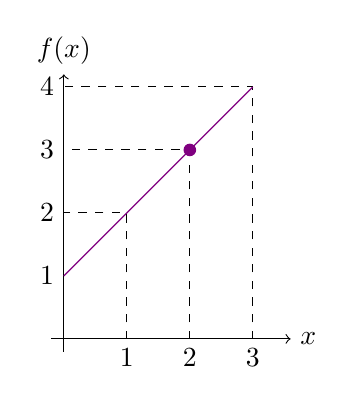
\begin{tikzpicture}[scale=0.8]
    \draw[->] (-0.2,0) -- (3.6,0) node[right] {$x$};
    \draw[->] (0,-0.2) -- (0,4.2) node[above] {$f(x)$};
    %
    \draw[dashed] (0,0) -- (0,1) node[left]{$1$};
    \draw[dashed] (1,0) node[below]{$1$} -- (1,2) -- (0,2) node[left]{$2$};
    \draw[dashed] (2,0) node[below]{$2$} -- (2,3) -- (0,3) node[left]{$3$};
    \draw[dashed] (3,0) node[below]{$3$} -- (3,4) -- (0,4) node[left]{$4$};
    %
    \draw[violet] (0,1) -- (3,4);
    \fill[violet] (2,3) circle[radius=1mm];
\end{tikzpicture}%Also used by abbildungen/04_abbildungen_in_koordinatensystemen
    }
    Der rechts abgebildete Graph gehört zur Abbildung \mbox{$f(x)=x+1$}. Der eingezeichnete Punkt hat die $x$-Koordinate $2$ und damit insgesamt die Koordinate $\coord{2}{f(2)}=\coord{2}{3}$. 
    
    Weil jedes Argument nur ein Bild haben kann, gibt es nur einen Punkt auf dem Graph von $f$, der den $x$-Wert $2$ hat.
    
    \picskip{3}
    Der Graph schneidet die $y$-Achse beim Wert $1$. Der dort liegende Punkt hat die $x$-Koordinate $0$ und insgesamt die Koordinate $\coord{0}{f(0)}=\coord{0}{1}$. Damit hat die Abbildung $f$ den $y$-Achsenabschnitt $1$.
    
    Der $y$-Achsenabschnitt von $f$ entspricht somit dem Wert $f(0)$ -- denn auf genau dieser Höhe liegt der Punkt über $x=0$, der die entsprechende Abbildungsvorschrift darstellt.
\end{example}

Um einen Abbildungsgraphen zu erhalten, hatten wir über jedem möglichen Argument (also jedem möglichen $x$-Wert) einen Punkt eingezeichnet. Jeder Punkt auf dem Abbildungsgraph steht für eine Abbildungsregel, die ein bestimmtes Argument auf ein bestimmtes Bild abbildet und hat die Koordinate $\coord{x}{f(x)}$ für ein $x\in\Real$.

Wir suchen nun einen Punkt, der auf dem Graphen einer Abbildung und gleichzeitig auch auf der $y$-Achse liegt. Jeder Punkt, der auf der $y$-Achse liegt, hat den $x$-Wert $0$ (die $y$-Achse geht nämlich vom Ursprung, dessen Koordinate $\coord{0}{0}$ ist, gerade nach oben und hat deshalb denselben $x$-Wert wie der Ursprung). 

Im Beispiel haben wir bereits gesehen, dass $\coord{0}{f(0)}$ der einzige Punkt auf dem Graphen ist, der auf der $y$-Achse liegt. Um den $y$-Achsenabschnitt einer beliebigen Abbildung auszurechnen, genügt es aus diesem Grund, einfach $f(0)$ zu berechnen.

\begin{example}{}
    \sloppy
    Die Abbildung $f(x)=4(x+1)$ hat den $y$-Achsenabschnitt $4$, denn um den $y$-Achsenabschnitt zu berechnen, muss einfach nur $f(0)$ berechnet werden. Es gilt $f(0)=4\cdot (0+1)=4$.
\end{example}

\fussy

\subsection{Nullstellen}
\label{sec:abbildungen_nullstelle}

Wie bereits beim $y$-Achsenabschnitt ist es, wenn man einen Graphe sieht, natürlich möglich, durch Hinsehen zu bestimmen, wo der Graph die $x$-Achse schneidet -- allerdings auch hier mit denselben Problemen. Um also zu \emph{berechnen}, wo ein Abbildungsgraph die $x$-Achse schneidet, müssen Punkte berechnet werden, deren $y$-Koordinate $0$ ist (das ist die Bedingung dafür, dass ein Punkt auf der $x$-Achse liegt).

Jeder Punkt auf dem Abbildungsgraphen hat die Koordinate $\coord{x}{f(x)}$, also eine Kombination aus einem Element $x$ aus der Definitionsmenge und dem Bild $f(x)$, auf das $x$ abgebildet wird. Damit die $y$-Koordinate $0$ wird, muss der rechte Teil, also $f(0)$, null werden. Für Schnittpunkte mit der $x$-Ache müssen deshalb einfach Werte für $x$ gefunden werden, für die $f(x)=0$ gilt.

\begin{example}{}
    \parpic[r]{
        \begin{tikzpicture}[samples=\ifdraft{5}{30}]
            \begin{axis}[defgrid, domain=0:4, y=.75cm, x=.75cm, xtick={1,...,4}, ytick={-1,...,3}, samples=\ifdraft{5}{20}]
                \addplot[color=violet] expression{(x-2)^2-1};
            \end{axis}
        \end{tikzpicture}
    }
    Rechts ist der Graph der Abbildung $f(x)=(x-2)^2-1$ abgebildet. Der Graph schneidet die $x$-Achse bei $x=1$ und $x=3$. 
    
    Das liegt daran, dass die Abbildung für beide $x$-Werte null wird: Es gilt \[f(3)=(3-2)^2-1=1-1=0\] und \[f(1)=(1-2)^2-1=1-1=0.\]
    
    \picskip{0}
    Wie du darauf kommen kannst, dass die Abbildung ausgerechnet an den Stellen $1$ und $3$ den Wert $0$ annimmt, ist zunächst nicht wichtig (das wird Gegenstand der Kapitel über lineare und quadratische Gleichungen sein).
    
    Weil der $y$-Wert eines Punktes auf dem Graphen immer $f(x)$ (also dem Bild eines gewissen Arguments) entspricht, ist liegt für diese beiden $x$-Werte der Punkt auf der $x$-Achse (denn der $y$-Wert ist $0$).
\end{example}

Der Graph einer Abbildung schneidet die $x$-Achse immer dann, wenn das Bild des betreffenden $x$-Wertes $0$ ist, also wenn $f(x)=0$ gilt. Wegen dieser Eigenschaft nennt man die $x$-Werte, für die eine Abbildung den Wert $0$ annimmt (und damit die $x$-Achse schneidet) auch \textbf{Nullstellen}.

\begin{definition}{Nullstelle\index{Nullstelle}}
    Ist $f$ eine Abbildung, dann heißen alle $x\in\Real$ mit $f(x)=0$ \textbf{Nullstellen} von $f$.
\end{definition}

Um herauszufinden, welche Werte man für $x$ wählen kann, damit $f(x)=0$ gilt, ist es nötig, eine Gleichung aufzulösen. $f(x)$ sollte dir immer in Form einer Berechnungsvorschrift vorliegen, z.B. in der Art \enquote{$f(x)=2x$}. Nun wäre es erforderlich, die Gleichung $2x=0$ aufzulösen, also alle $x$ zu finden, für die $2x=0$ gilt. 

Das lernst du vor allem in den Kapiteln über \textbf{lineare und quadratische Gleichungen}. Zunächst wird es nicht erforderlich sein, dass du systematisch Gleichungen lösen kannst -- stattdessen werden die Nullstellen in der Regel so einfach sein, dass sie sich leicht durch Ausprobieren finden lassen.

\begin{example}{}
    Die Nullstellen der Abbildung $f(x)=x+5$ sind alle Werte, die sich für $x$ einsetzen lassen, damit $f(x)=0$ gilt. Es muss die Gleichung $\colorbrace{x+5}{f(x)}=0$ gelöst werden. Der einzige Wert, den man für $x$ wählen kann, damit $f(x)=x+5=0$ gilt, ist $x=-5$.
    
    Es folgt, dass $f$ genau eine Nullstelle hat, und zwar bei $x=-5$.
\end{example}

\begin{nutshell}{Nullstellen und $y$-Achsenabschnitt}
    Die Schnittpunkte eines Abbildungsgraphen mit den beiden Koordinatenachsen (also der $x$-Achse und der $y$-Achse) werden besonders bezeichnet.
    
    Ein Schnittpunkt des Graphen einer Abbildung $f$ mit der $x$-Achse wird als \textbf{Nullstelle} von $f$ bezeichnet, weil die Abbildung hier den Wert 0 hat: Damit der Graph die $x$-Achse an einem Punkt $\coord{x}{0}$ schneidet, muss $f(x)=0$ sein. Grundsätzlich kann eine Abbildung mehrere Nullstellen haben, nämlich dann, wenn es mehrere verschiedene Werte für $x$ gibt, sodass $f(x)=0$ gilt.
    
    Ein Schnittpunkt des Graphen von $f$ mit der $y$-Achse heißt \textbf{$y$-Achsenabschnitt} von $f$. Jede Abbildung hat nur einen $y$-Achsenabschnitt, weil jeder Punkt auf der $y$-Achse eine Koordinate $\coord{0}{y}$ haben muss, deren $x$-Wert 0 ist. Der $y$-Achsenabschnitt ist genau der Wert $f(0)$, weil das die einzige Abbildungsregel ist, die einen Punkt auf der $y$-Achse erzeugen kann.
\end{nutshell}

\end{document}